% 
% Author: Bratin Mondal
% Roll No: 21CS10016
% Department of Computer Science and Engineering
% Indian Institute of Technology, Kharagpur
%

\documentclass[12pt]{article}
\usepackage{amsmath, amssymb, graphicx}
\usepackage{amsthm}  
\usepackage{float} 
\usepackage{geometry}
\usepackage{hyperref} 
\usepackage{cleveref}
\usepackage{algorithm}
\usepackage{algorithmic}
\usepackage[backend=biber,style=ieee]{biblatex}
\addbibresource{references.bib} 

\geometry{a4paper, top=0.25in, bottom=0.25in, left=0.25in, right=0.25in}  

\title{Computational Geometry (CS60064)\\ Homework Set 3}
\author{
    Bratin Mondal - 21CS10016
}
\date{}

\newtheorem{claim}{Claim} 

\begin{document}
\maketitle

\section*{Question 1}
The diameter of a convex polygon is a/the longest line segment contained within it. Given a convex polygon \( P \) with \( n \) vertices in counterclockwise order, design an \( O(n) \)-time algorithm to find a diameter of \( P \). Justify its correctness and why its time complexity is \( O(n) \).

\section*{Solution}
Let us assume that the convex polygon is given in the form of a list of vertices in counterclockwise order. Let the vertices be denoted by \( p_1, p_2, \ldots, p_n \) where \( p_i = (x_i, y_i) \) for \( 1 \leq i \leq n \).

\subsection*{Description of the Algorithm}

The algorithm to compute the diameter efficiently in \( O(n) \) time is as follows:

\begin{algorithm}[H]
\caption{Compute the diameter of a convex polygon}
\begin{algorithmic}[1]
\STATE $i \leftarrow n$
\STATE $j \leftarrow i + 1$
\WHILE {\texttt{Area}$(p_i, p_{i+1}, p_{j+1})$ \textgreater{} \texttt{Area}$(p_i, p_{i+1}, p_j)$}
    \STATE $j \leftarrow j + 1$
\ENDWHILE
\STATE $j_0 \leftarrow j$
\STATE Initialize an empty vector $pairs$
\WHILE {$i \neq j_0$}
    \STATE $i \leftarrow i + 1$
    \STATE Add $(i, j)$ to $pairs$
    \WHILE {\texttt{Area}$(p_i, p_{i+1}, p_{j+1})$ \textgreater{} \texttt{Area}$(p_i, p_{i+1}, p_j)$}
        \STATE $j \leftarrow j + 1$
        \IF {$(i, j) \neq (j_0, 1)$}
            \STATE Add $(i, j)$ to $pairs$
        \ENDIF
    \ENDWHILE
    \IF {\texttt{Area}$(p_i, p_{i+1}, p_{j+1}) = \texttt{Area}(p_i, p_{i+1}, p_j)$}
        \IF {$(i, j) \neq (j_0, n)$}
            \STATE Add $(i, j+1)$ to $pairs$
        \ENDIF
    \ENDIF
\ENDWHILE
\STATE Compute the maximum Euclidean distance between points in $pairs$
\STATE Return the pair of points with the maximum distance
\end{algorithmic}
\end{algorithm}

The function \texttt{Area} computes the area of the triangle formed by three points \( p_i, p_j, p_k \) using the determinant formula:
\begin{equation}
    \texttt{Area}(p_i, p_j, p_k) = \frac{1}{2} \left| x_i(y_j - y_k) + x_j(y_k - y_i) + x_k(y_i - y_j) \right|
\end{equation}

The above algorithm efficiently finds all antipodal pairs using the rotating calipers method and then determines the pair with the maximum Euclidean distance, which represents the diameter of the convex polygon.

\subsection*{Correctness of the Algorithm}

Consider a vertex \( p_i \) of the convex polygon. Suppose we traverse the counterclockwise chain along the boundary of \( P \) starting at \( p_i \), until we reach a vertex \( q_R^{(i)} \), which is the farthest vertex from \( p_{i-1}p_i \). In case of ties, when \( P \) has parallel edges, \( q_R^{(i)} \) is the first vertex encountered in this traversal. Similarly, we define \( q_L^{(i)} \) as the vertex farthest from \( p_ip_{i+1} \) in the clockwise traversal of the boundary of \( P \) starting at \( p_i \).

We first claim that the chain of vertices between \( q_R^{(i)} \) and \( q_L^{(i)} \) defines the set \( C(p_i) \) of vertices that form an antipodal pair with \( p_i \). To prove this claim, we first derive the condition for a set of vertices to be antipodal.

\begin{figure}[H]
    \centering
    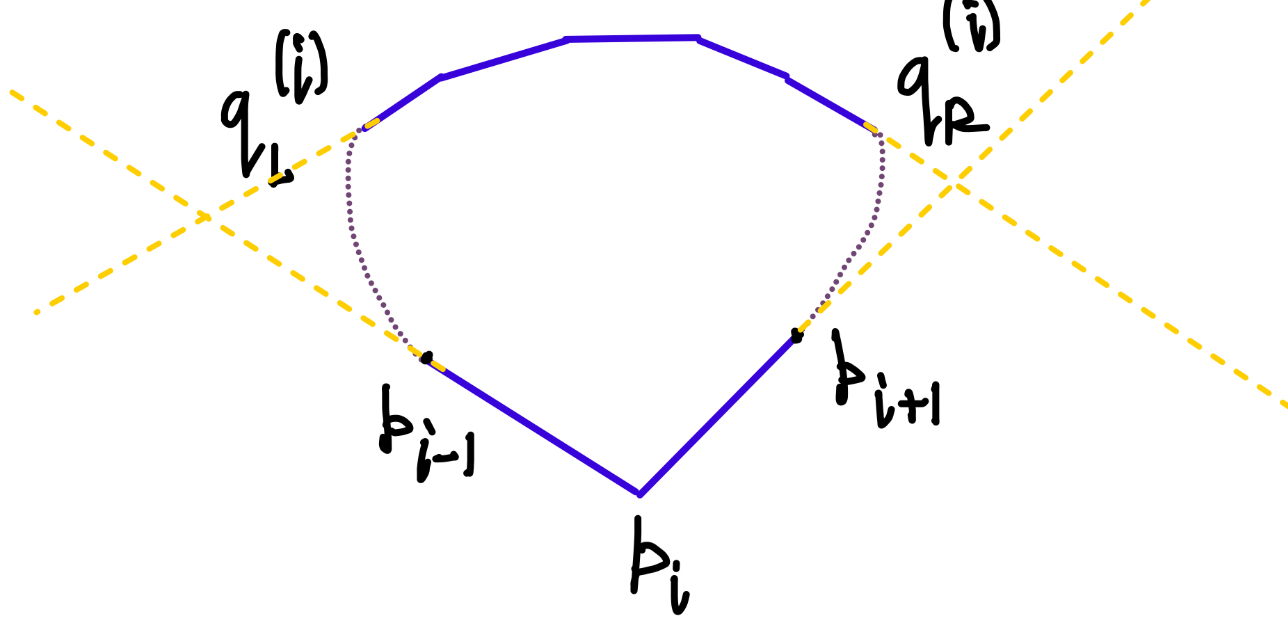
\includegraphics[width=0.5\textwidth]{img/1.jpg}
    \caption{Antipodal pairs for a vertex \( p_i \)}
    \label{fig:1}
\end{figure}

Consider two vertices \( p_i \) and \( p_j \). Let \( \alpha_i \) denote the external angle formed by the line segment \( p_{i-1} p_i \) and \( p_i p_{i+1} \), and let \( \alpha_j \) denote the external angle formed by the line segment \( p_{j-1} p_j \) and \( p_j p_{j+1} \). The pair of vertices \( p_i \) and \( p_j \) are antipodal if and only if there is a straight line in the intersection of \( \alpha_i \) and \( \alpha_j \). Informally, we can say that \( \alpha_i \) and \( \alpha_j \) should overlap in two opposite directions; just one intersection is not sufficient for a line to pass through.

\begin{figure}[H]
    \centering
    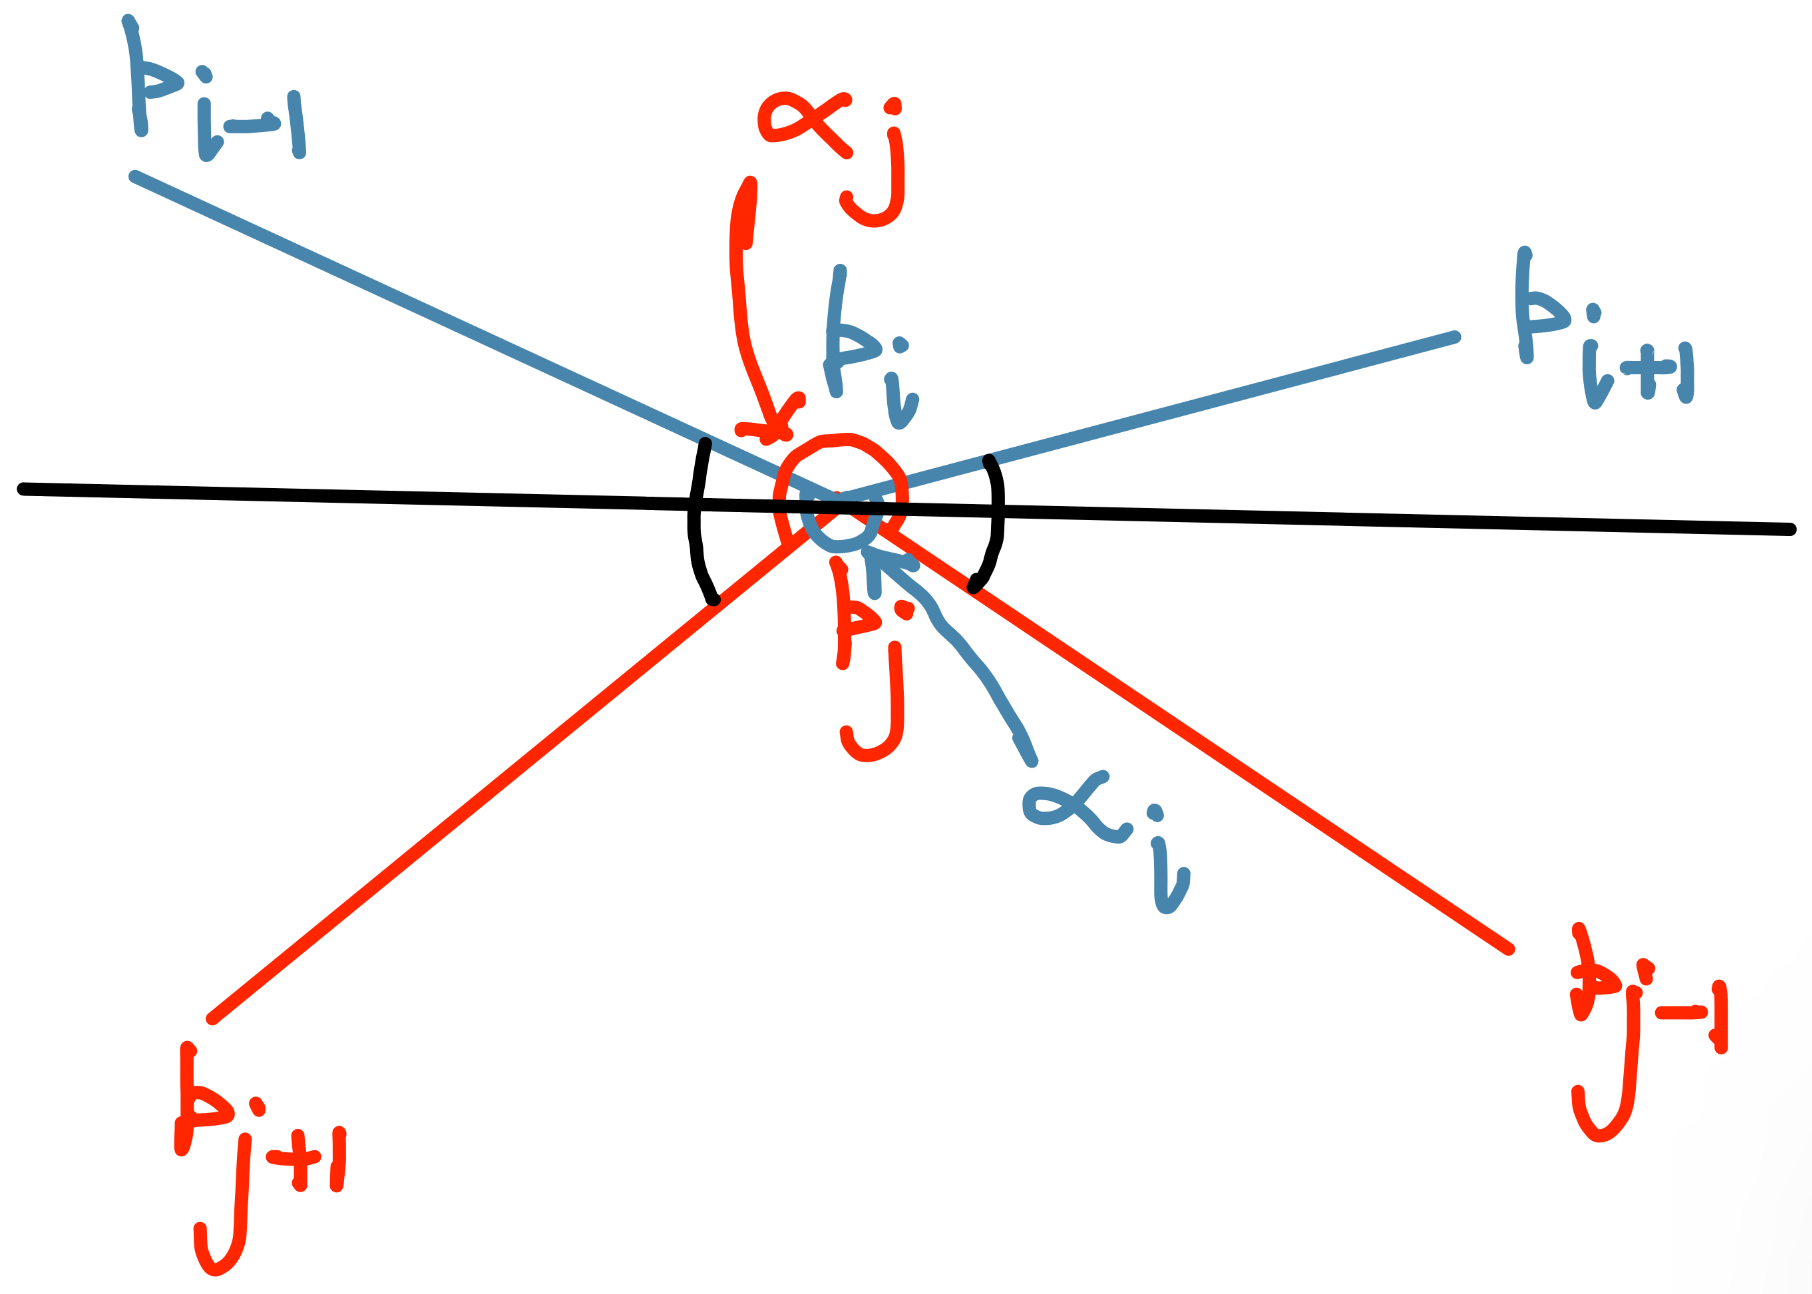
\includegraphics[width=0.5\textwidth]{img/2.jpg}
    \caption{Condition for antipodal pairs}
    \label{fig:2}
\end{figure}

We now prove that during our counterclockwise traversal of the boundary of \( P \) starting at \( p_i \), any vertex before \( q_R^{(i)} \) or after \( q_L^{(i)} \) cannot be part of an antipodal pair with \( p_i \). Consider the vertex \( p_j \) encountered just before \( q_R^{(i)} \) during the traversal. Through the point \( q_R^{(i)} \), draw a line parallel to \( p_{i-1} p_i \) and call it \( L_{q_R^{(i)}} \). Since \( q_R^{(i)} \) is the farthest vertex from \( p_{i-1} p_i \), the point \( p_j \) must lie on the same side of the line as \( p_i \). Let the segment \( q_R^{(i)} p_j \) form an angle \( \alpha \) (\( \alpha > 0 \)) with \( L_{q_R^{(i)}} \). The same angle \( \alpha \) is formed by \( q_R^{(i)} p_j \) with any line segment parallel to \( p_{i-1} p_{i} \). Due to this, the intersection of \( \alpha_i \) and \( \alpha_j \) cannot contain a straight line, since it will only have one intersection. There cannot be another intersection, as \( \alpha \) represents the opposite non-overlapping part. Hence, \( p_j \) cannot be part of an antipodal pair with \( p_i \). (As shown in \Cref{fig:3}, \(\alpha_{i} \cap \alpha_j\) has only one intersection and a straight line cannot pass through it.) 

Due to the convex nature of angles, any other vertex before \( p_j \) will also not be part of an antipodal pair with \( p_i \). Similarly, we can prove that any vertex after \( q_L^{(i)} \) cannot be part of an antipodal pair with \( p_i \). Due to convex nature of \(C(p_i)\), the set of vertices between \( q_R^{(i)} \) and \( q_L^{(i)} \) (inclusive) forms the antipodal pair with \( p_i \).

\begin{figure}[H]
    \centering
    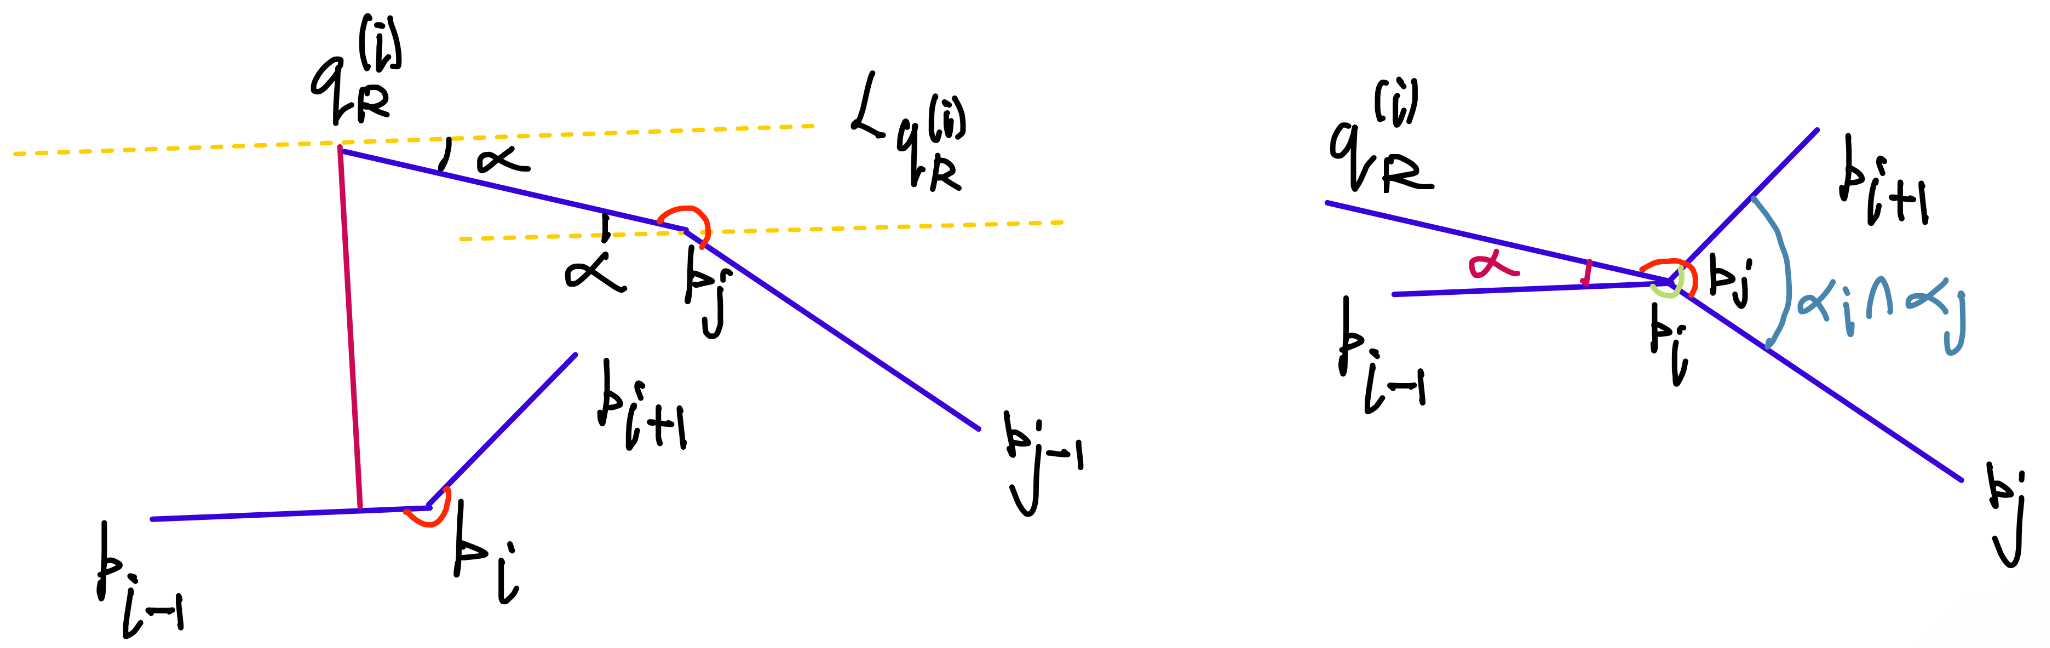
\includegraphics[width=1\textwidth]{img/3.jpg}
    \caption{Vertex before \( q_R^{(i)} \) cannot be part of the antipodal pair with \( p_i \)}
    \label{fig:3}
\end{figure}

The proposed algorithm efficiently finds the antipodal pairs for all vertices of the convex polygon. Lines 1-4 locate the vertex \(q_R^{(1)}\). The subsequent while loop which constructs the set \(C(p_{i})\) uses two pointers \(i\) and \(j\) to traverse the vertices of the polygon. These two pointers move counterclockwise around \(P\), \(i\) advancing from \(n\) to \(q_R^{(1)}\) and \(j\) advancing from \(q_R^{(1)}\) to \(n\). An antipodal pair is generated each time any of the pointers advances. Parallel edges which can lead to a point having multiple antipodal pairs are handled by lines 17-21. The first pair generated is \(p_1, p_{j_0}\) and the last pair generated is \(p_{j_0}, p_n\). Hence, each antipodal pair is generated exactly once since \(i\) advances from \(1\) to \(j_0\) and \(j\) advances from \(j_0\) to \(n\). Finally, the pair of points with the maximum Euclidean distance is returned as the diameter of the convex polygon.

\subsection*{Time Complexity Analysis}

Finding \(j_0\) in lines 1--4 takes \(O(n)\) time. Since each antipodal pair is generated exactly once as \(i\) advances from \(1\) to \(j_0\) and \(j\) advances from \(j_0\) to \(n\), the while loop consists of a total of \(n\) moves. Hence, the while loop takes \(O(n)\) time.

In the absence of parallel edges, the while loop generates exactly \(n\) antipodal pairs. If parallel edges exist, their number is at most \(\lfloor n/2 \rfloor\), resulting in a maximum of \(3n/2\) antipodal pairs.

The final step of computing the maximum Euclidean distance among the pairs takes \(O(n)\) time. Thus, the overall time complexity of the algorithm is \(O(n)\).


\section*{Question 2}


Let \( P \) and \( Q \) be two convex polygons with \( m \) and \( n \) vertices, respectively, given in counterclockwise order.   Suggest an \( O(m \log n) \)-time algorithm to check whether \( P \) contains \( Q \). Suggest another algorithm that will take time \( O(m + n) \). Derive the time complexities of both algorithms.

\section*{Solution}
Let the vertices of the convex polygon \( P \) be denoted by \( p_1, p_2, \ldots, p_m \) and the vertices of the convex polygon \( Q \) be denoted by \( q_1, q_2, \ldots, q_n \).

\subsubsection*{Part-1}

Deriving an algorithm with a time complexity of \( O(n \log m) \) is straightforward. For each point in \( Q \), we can use the convex polygon membership query algorithm to check if the point lies inside \( P \), where each query takes \( O(\log m) \) time (as discussed in Homework 1). If all points in \( Q \) are inside \( P \), then due to the convex nature of \( Q \), \( Q \) is completely inside \( P \). The total time complexity of this algorithm is therefore \( O(n \log m) \).

For an algorithm with \( O(m \log n) \) time complexity, we will use a different approach where for every edge of \( P \), we check if the vertices of \( Q \) lie on the same side as the vertices of \( P \).

Specifically, for each edge of \( P \), we proceed as follows. Let \( p_i p_{i+1} \) be the current edge of \( P \). First, we consider the perpendicular direction to the edge \( p_i p_{i+1} \), which points towards the interior of the polygon. We then consider a line passing through the midpoint of the edge \( p_i p_{i+1} \) in this perpendicular direction. Let this line be denoted by \( \vec{p}_{\perp} \), and the midpoint of the edge \( p_i p_{i+1} \) is \( p_{\text{mid}} \).

Next, consider the projection of all the vertices of \( Q \) onto the line \( \vec{p}_{\perp} \). We note that we do not need to construct all the projection points, but we compute them on the fly as needed. The \texttt{projection distance} for a projection point \( q_j \) on the line \( \vec{p}_{\perp} \) is defined as the \texttt{signed distance} of the projection point from the midpoint \( p_{\text{mid}} \) of the edge \( p_i p_{i+1} \). The \texttt{signed distance} is positive if the projection point is on the side of the edge \( p_i p_{i+1} \) that is the interior of the polygon and negative otherwise.

\begin{figure}[H]
    \centering
    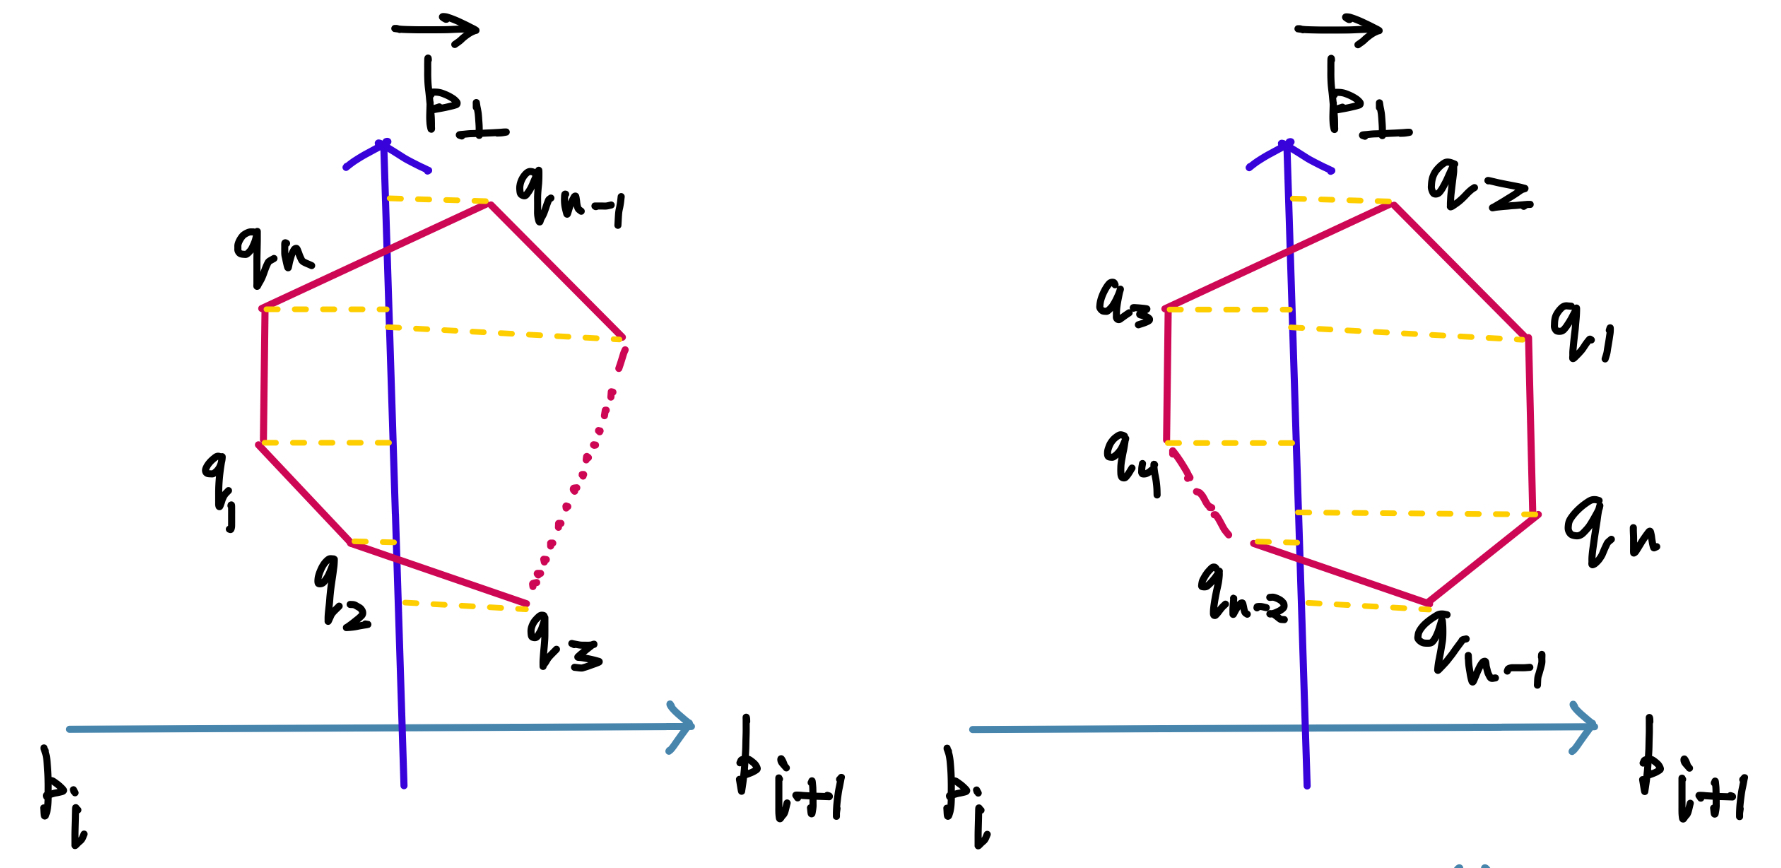
\includegraphics[width=0.8\textwidth]{img/4.jpg}
    \caption{Projection of vertices of \( Q \) on the line \( \vec{p}_{\perp} \)}
    \label{fig:4}
\end{figure}

We observe that due to the convex nature of \( Q \), the \texttt{projection distance} of the vertices of \( Q \) on the line \( \vec{p}_{\perp} \) can follow two specific patterns. The first pattern decreases to a minimum, increases to a maximum, and then decreases again. The second pattern increases to a maximum, decreases to a minimum, and then increases again. (Any of the increasing or decreasing parts can have length 0.) The comparison between the \texttt{projection distance} of \( q_1 \) and \( q_n \) will tell us which pattern we are dealing with. If the \texttt{projection distance} of \( q_1 \) is less than that of \( q_n \), we are in the first pattern; otherwise, we are in the second pattern.

Now, we can perform a binary search to find the minima and maxima of the \texttt{projection distance} of the vertices of \( Q \) on the line \( \vec{p}_{\perp} \) in \( O(\log n) \) time. The binary search algorithm needs to be modified to work in the presence of the two types of increasing/decreasing patterns.

For simplicity, we describe the binary search approach for the first pattern. As shown in \Cref{fig:5}, there are two decreasing regions labeled \( C_{\text{dec}}^1 \) and \( C_{\text{dec}}^2 \), and one increasing region labeled \( C_{\text{inc}} \). It is clear that we can easily detect when we are in \( C_{\text{inc}} \) during the binary search and can move left for a minimum and right for a maximum. To distinguish between \( C_{\text{dec}}^1 \) and \( C_{\text{dec}}^2 \), we compare the \texttt{projection distance} of the current element with \( q_1 \). If it is greater, we are in \( C_{\text{dec}}^2 \); otherwise, we are in \( C_{\text{dec}}^1 \), and we move accordingly for the binary search. The second pattern can be handled similarly.

\begin{figure}[H]
    \centering
    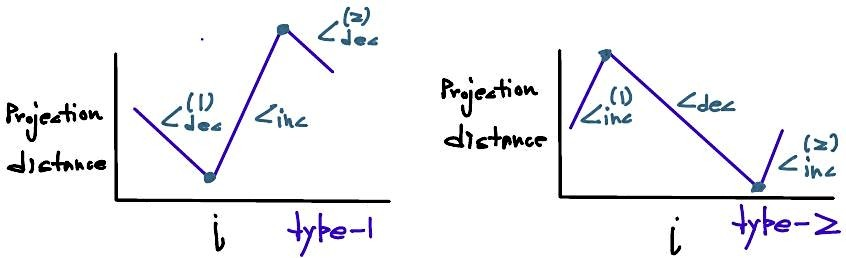
\includegraphics[width=0.8\textwidth]{img/5.jpg}
    \caption{Finding the maxima of the \texttt{projection distance} of the vertices of \( Q \) on the line \( \vec{p}_{\perp} \)}
    \label{fig:5}
\end{figure}

We are interested in finding the minima in this case. Using the approach described above, we find the minima of the \texttt{projection distance} of the vertices of \( Q \) on the line \( \vec{p}_{\perp} \). If we find a minimum that is less than 0, we can conclude that \( Q \) is not completely inside \( P \). (We can include other optimizations, such as immediately concluding that \( Q \) is not inside \( P \) if we find any \texttt{projection distance} less than 0 during the binary search, but this does not improve the time complexity.)

Thus, in the final algorithm, we check for all edges of \( P \). If we find a minimum less than 0 for any edge, we can conclude that \( Q \) is not completely inside \( P \). If no such minimum is found, we conclude that \( Q \) is completely inside \( P \).

\subsubsection*{Time Complexity Analysis}
For each edge of \( P \), we perform a binary search to find the minima of the \texttt{projection distance} of the vertices of \( Q \) on the line \( \vec{p}_{\perp} \). We compute the \texttt{projection distance} of the vertices of \( Q \) on the fly as needed which helps us avoid computing all the projection points. The binary search takes \( O(\log n) \) time. Since there are \( m \) edges in \( P \), the total time complexity of the algorithm is \( O(m \log n) \).

\subsubsection*{Part-2}
To check whether polygon \( Q \) is completely inside polygon \( P \) in \( O(m + n) \) time, we apply the convex polygon intersection algorithm described in \cite{OROURKE1982384}. The idea is to construct the intersection of the two polygons and verify if the intersection is equal to \( Q \). The time complexity of this algorithm is \( O(m + n) \). 

We begin by defining some necessary terms. For a point \( p_{i} \) in a polygon \( P \), the half-plane \( hp(p_{i}) \) is defined as the set of points that lie on the same side as the other points of the polygon with respect to the line passing through vertices \( p_{i-1} \) and \( p_{i} \). The mathematical definition of \( hp(p_{i}) \) is given by:
\[
hp(p_{i}) = \{ p \in \mathbb{R}^{2} : (p_{i} - p_{i-1}) \times (p - p_{i}) \geq 0 \}
\]
where \( \times \) denotes the cross product of two vectors.

The algorithm for finding the intersection of two convex polygons is described in \Cref{alg:2}. The process begins with the first vertices of the two polygons and iterates over the vertices of both polygons. Depending on the relative position of the vertices, the algorithm advances through the vertices and calculates the intersection points. The algorithm terminates after at most \( 2(|P| + |Q|) \) iterations, after which we can conclude that the polygons do not intersect. 

Subsequently, the algorithm checks if one of the polygons is completely inside the other by verifying if all vertices of one polygon lie on the same side of all edges of the other polygon. If one polygon is fully contained within the other, the algorithm outputs the polygon that is completely inside. If neither polygon is fully contained within the other, the algorithm outputs \( \varnothing \).


\begin{algorithm}[H]
    \caption{Intersection of two convex polygons} \label{alg:2}
    \begin{algorithmic}[1]
    \STATE $p \leftarrow p_1$, $q \leftarrow q_1$ and \( \texttt{intersection\_polygon} \leftarrow \emptyset \)
    \REPEAT
        \STATE {Test if $p$ and $q$ intersect}
        \IF{$p$ and $q$ intersect}
            \IF{this intersection is the same as the first intersection}
                \STATE {output \texttt{intersection\_polygon}}
            \ELSE
                \STATE {add the intersection point to \texttt{intersection\_polygon}}
                \IF{$p \in hp(q)$}
                    \STATE inside $\gets$ ``P"
                \ELSE
                    \STATE inside $\gets$``Q"
                \ENDIF
            \ENDIF
        \ENDIF
        \IF{$q \times p \geq 0$}
            \IF{$p \in hp(q)$}
                \STATE \texttt{advance} $q$
            \ELSE
                \STATE \texttt{advance} $p$
            \ENDIF
        \ELSE
            \IF{$q \in hp(p)$}
                \STATE \texttt{advance} $p$
            \ELSE
                \STATE \texttt{advance} $q$
            \ENDIF
        \ENDIF
    \UNTIL{repeat has executed more than $2(|P| + |Q|)$ times}
    \STATE \(p \leftarrow p_1\), \(q \leftarrow q_1\)
    \IF{$p \in Q$ (By checking if $p$ lies on the same side of all edges of $Q$)}
        \STATE output P
    \ELSIF{$q \in P$ (By checking if $q$ lies on the same side of all edges of $P$)}
        \STATE output Q
    \ELSE
        \STATE output \(\varnothing\)
    \ENDIF
\end{algorithmic}
\end{algorithm}

The \texttt{advance} operation is defined as follows for a point \(p_{i}\) in a polygon \(P\):

\begin{algorithm}[H]
    \caption{Advance \(p_{i}\) for polygon \(P\)}
    \begin{algorithmic}[1]
    \IF{\texttt{inside} = ``P"}
        \STATE add \(p_{i}\) to \texttt{intersection\_polygon}
    \ENDIF
    \STATE \(i \leftarrow (i \mod |P|) + 1\)
\end{algorithmic}
\end{algorithm}

Similarly, the \texttt{advance} operation for a point \(q_{i}\) in a polygon \(Q\) is defined as follows:

\begin{algorithm}[H]
    \caption{Advance \(q_{i}\) for polygon \(Q\)}
    \begin{algorithmic}[1]
    \IF{\texttt{inside} = ``Q"}
        \STATE add \(q_{i}\) to \texttt{intersection\_polygon}
    \ENDIF
    \STATE \(i \leftarrow (i \mod |Q|) + 1\)
\end{algorithmic}
\end{algorithm}

Our final algorithm for checking if \(Q\) is completely inside \(P\) operates in \(O(m + n)\) time. It first computes the intersection of the two polygons using \Cref{alg:2}. If the intersection is equal to \(Q\), then \(Q\) is completely inside \(P\). 

Note that the original algorithm for computing the intersection also checks if one polygon is completely inside the other. However, in cases where \(Q\) is inside \(P\) and their edges overlap, we still need to find the intersection to verify that \(Q\) is completely inside \(P\).

\subsection*{Time Complexity Analysis}

The algorithm iterates over the vertices of the two polygons. The repeat loop executes at most \(2(|P| + |Q|)\) times. If the two polygons do not intersect, the algorithm terminates after at most \(2(|P| + |Q|)\) iterations. In this case, we only need to check if one polygon is completely inside the other, which takes \(O(m + n)\) time.

The intersection of the two polygons can have at most \(m + n\) vertices. This is because every edge of \(P\) can be separated into at most three parts by the edges of \(Q\), but at most one of these parts can be part of the intersection. The same reasoning applies to the edges of \(Q\).

To check if the intersection is equal to \(Q\), we first verify if \(q_1\) exists in the intersection. This can be done in \(O(m+n)\) time. Once \(q_1\) is found, we compare the vertices of \(Q\) with the vertices of the intersection, which also takes \(O(m+n)\) time.

Hence, the total time complexity of the algorithm is \(O(m + n)\).


\printbibliography

\end{document}

